\documentclass[12pt,a4paper]{article}

\usepackage[utf8]{inputenc}
\usepackage[T1]{fontenc}
\usepackage[italian]{babel}
\usepackage{geometry}
\usepackage{graphicx}
\usepackage{float}
\usepackage{array}
\usepackage{longtable}
\usepackage{booktabs}
\usepackage{hyperref}
\usepackage{xcolor}
\usepackage{titlesec}
\usepackage{fancyhdr}
\usepackage{enumitem}
\usepackage{caption}
\usepackage{needspace}
\usepackage{tabularx}
\usepackage{xurl}

\newcolumntype{L}[1]{>{\raggedright\arraybackslash}m{#1}}

\geometry{
    top=2.5cm,
    bottom=2.5cm,
    left=2.5cm,
    right=2.5cm
}

\hypersetup{
    colorlinks=true,
    linkcolor=blue,
    urlcolor=blue,
    citecolor=blue
}

\pagestyle{fancy}
\fancyhf{}
\lhead{BugBoard26}
\rhead{Documento di design}
\cfoot{Pagina \thepage}

\titleformat{\section}
{\normalfont\Large\bfseries\color{blue!40!black}}
{\thesection}{1em}{}

\titleformat{\subsection}
{\normalfont\large\bfseries\color{blue!35!black}}
{\thesubsection}{1em}{}

\setlist[itemize]{topsep=4pt,itemsep=2pt}
\setlist[enumerate]{topsep=4pt,itemsep=2pt}

\begin{document}

\begin{titlepage}
    \centering
    \vspace*{2cm}

    {\Huge \textbf{BugBoard26}\par}
    \vspace{0.5cm}
    {\Large Documento di design del sistema\par}

    \vspace{1.5cm}

    {\large Progetto di Ingegneria del Software\par}
    {\large A.A. 2025/2026\par}

    \vfill

    \begin{tabular}{ll}
        \textbf{Componenti} & Valerio Porcile, Emanuel Giuseppe Lupoli, Emanuele Martucci \\
        \textbf{Modalità} & Tradizionale \\
        \textbf{Versione} & 1.0 \\
        \textbf{Data} & \today \\
    \end{tabular}

    \vfill
\end{titlepage}

\tableofcontents
\clearpage

\section{Introduzione}

Il presente documento descrive la progettazione del sistema BugBoard26, realizzato come applicazione distribuita per la gestione collaborativa di issue in progetti software.

Il documento rappresenta la seconda fase del lavoro progettuale e riprende quanto definito nella specifica dei requisiti. In particolare, vengono descritte le scelte architetturali, la suddivisione delle responsabilità tra frontend, backend e database, la struttura principale delle classi di design e le motivazioni delle principali scelte tecnologiche.

Le funzionalità considerate sono quelle assegnate al gruppo:

\begin{itemize}
    \item autenticazione tramite email e password;
    \item creazione di utenti da parte degli amministratori;
    \item creazione di issue da parte degli utenti autenticati;
    \item visualizzazione, ricerca, filtro e ordinamento delle issue;
    \item cambio stato delle issue assegnate;
    \item notifica al segnalatore quando una issue viene risolta;
    \item esportazione delle issue in formato CSV;
    \item archiviazione delle issue da parte degli amministratori;
    \item suggerimento automatico dello assegnatario in base al carico di lavoro;
    \item gestione di utenti readonly;
    \item contrassegno di una issue come duplicata.
\end{itemize}

\section{Obiettivi di progettazione}

La progettazione del sistema è stata guidata dai seguenti obiettivi:

\begin{itemize}
    \item separare chiaramente frontend, backend e persistenza;
    \item mantenere il backend indipendente dalla tecnologia utilizzata per la interfaccia utente;
    \item esporre le funzionalità tramite API REST;
    \item centralizzare la logica applicativa nel backend;
    \item applicare una struttura a livelli, distinguendo controller, servizi, repository e persistenza;
    \item limitare la complessità, mantenendo il sistema coerente con il lavoro di un gruppo di tre studenti;
    \item rendere il progetto facilmente testabile, estendibile e spiegabile in sede di discussione.
\end{itemize}

\section{Architettura generale}

Il sistema è stato progettato come applicazione web distribuita composta da tre macro componenti:

\begin{itemize}
    \item \textbf{Frontend Angular}, responsabile della interfaccia utente e della interazione con lo utente;
    \item \textbf{Backend ASP.NET Core Web API}, responsabile della logica applicativa, della autenticazione, della gestione dei ruoli e della esposizione delle API REST;
    \item \textbf{Database PostgreSQL}, responsabile della persistenza dei dati.
\end{itemize}

La comunicazione tra frontend e backend avviene esclusivamente tramite richieste HTTP verso API REST. Le richieste protette includono un token JWT generato dal backend durante la fase di login.

Questa scelta permette di rispettare il vincolo di separazione tra frontend e backend: il backend non dipende da Angular e potrebbe essere utilizzato anche da una diversa interfaccia, per esempio una applicazione mobile o desktop.

\Needspace{10\baselineskip}
\subsection{Component diagram}

Il component diagram mostra la suddivisione logica del sistema. Il frontend contiene i componenti grafici e i servizi Angular che invocano le API del backend. Il backend è organizzato in controller, servizi applicativi, repository e DbContext. Il database contiene le tabelle principali del sistema.

\IfFileExists{diagrammi_architetturali/component_diagram.png}{
\begin{figure}[H]
    \centering
    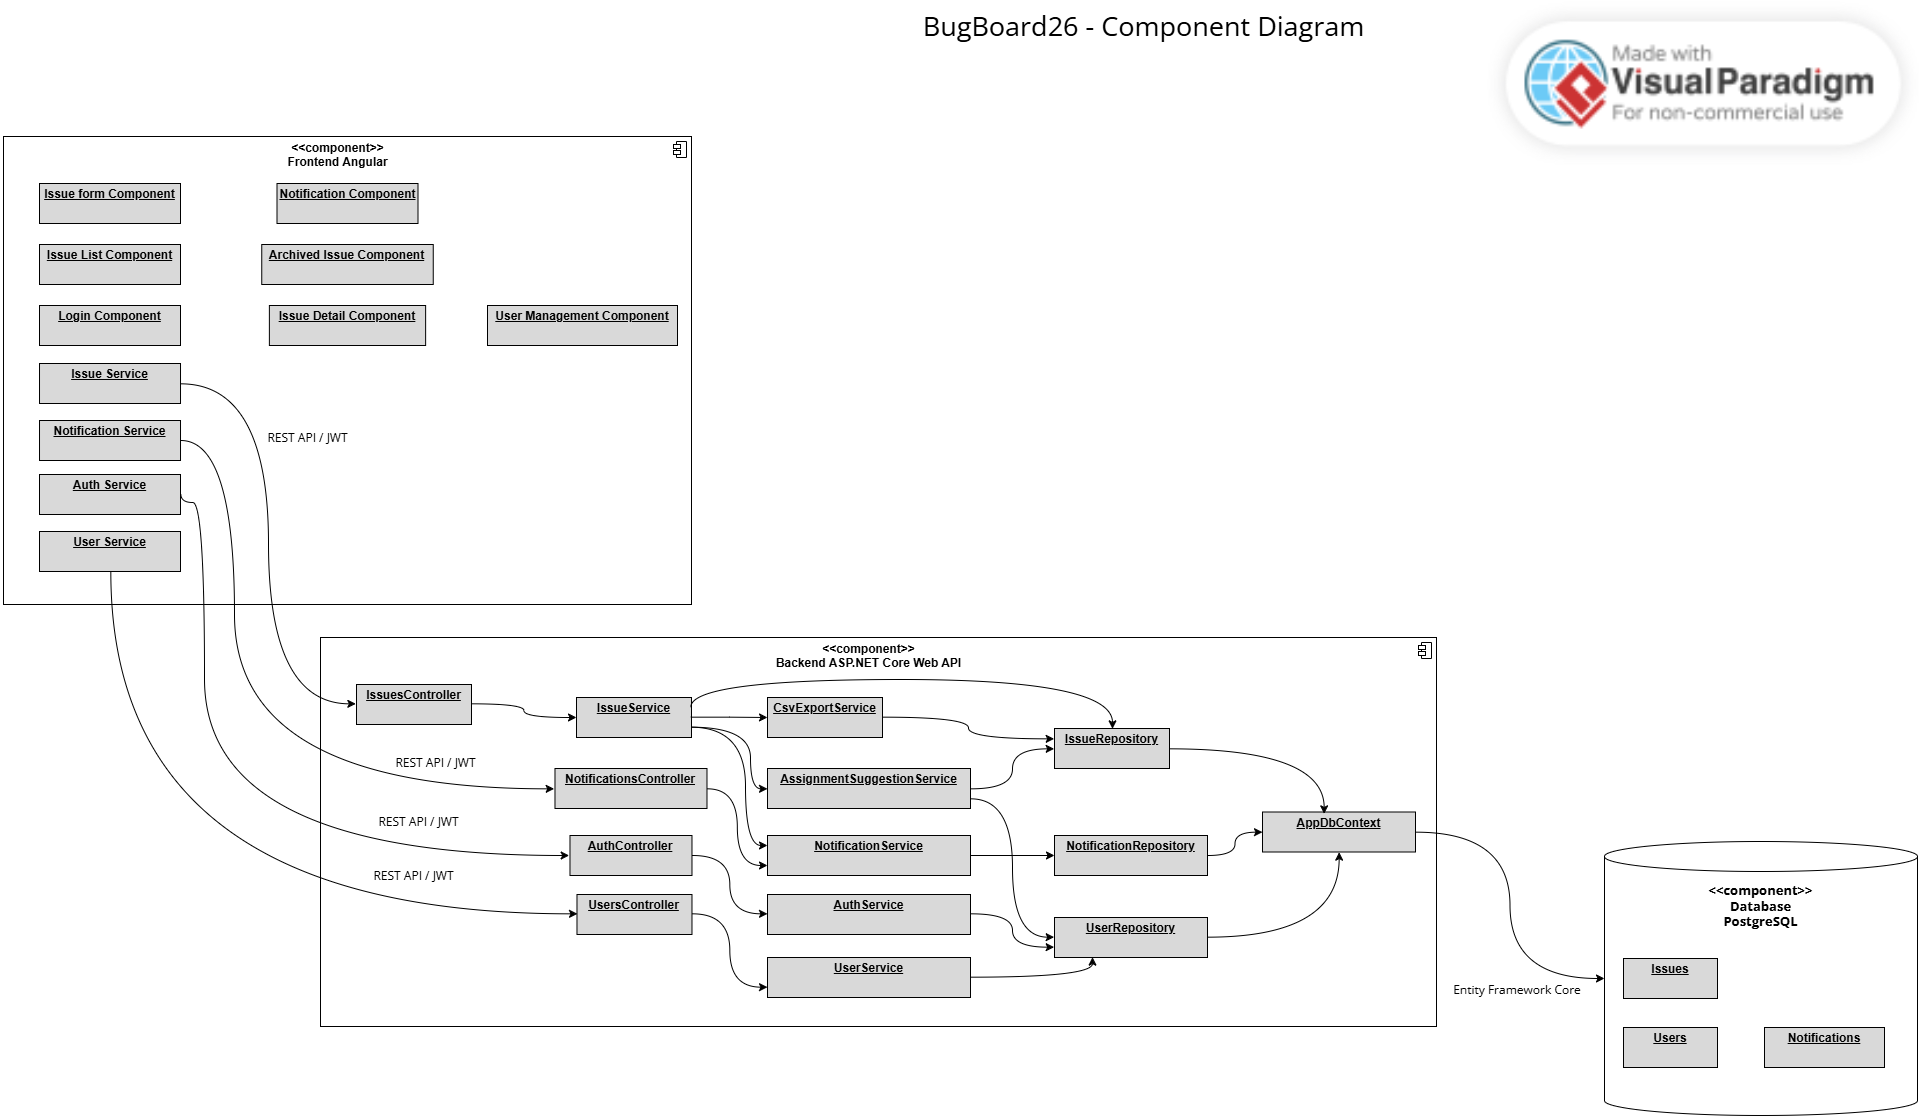
\includegraphics[width=0.95\textwidth]{diagrammi_architetturali/component_diagram.png}
    \caption{Component diagram di BugBoard26}
    \label{fig:component-diagram}
\end{figure}
}{
\begin{center}
    \fbox{\parbox{0.85\textwidth}{
        \centering
        Il file \texttt{diagrammi\_architetturali/component\_diagram.png} non è stato trovato.
    }}
\end{center}
}

Nel diagramma sono evidenziate le principali dipendenze tra i componenti: il frontend comunica con i controller del backend tramite API REST e JWT, i controller delegano la logica ai servizi, i servizi utilizzano repository e il livello di persistenza accede al database tramite Entity Framework Core.

\Needspace{10\baselineskip}
\subsection{Deployment diagram}

Il deployment diagram mostra una possibile distribuzione del sistema. Lo utente accede alla applicazione tramite browser. La parte frontend comunica con il backend tramite rete, mentre il backend accede al database PostgreSQL tramite protocollo PostgreSQL.

\IfFileExists{diagrammi_architetturali/deployment_diagram.png}{
\begin{figure}[H]
    \centering
    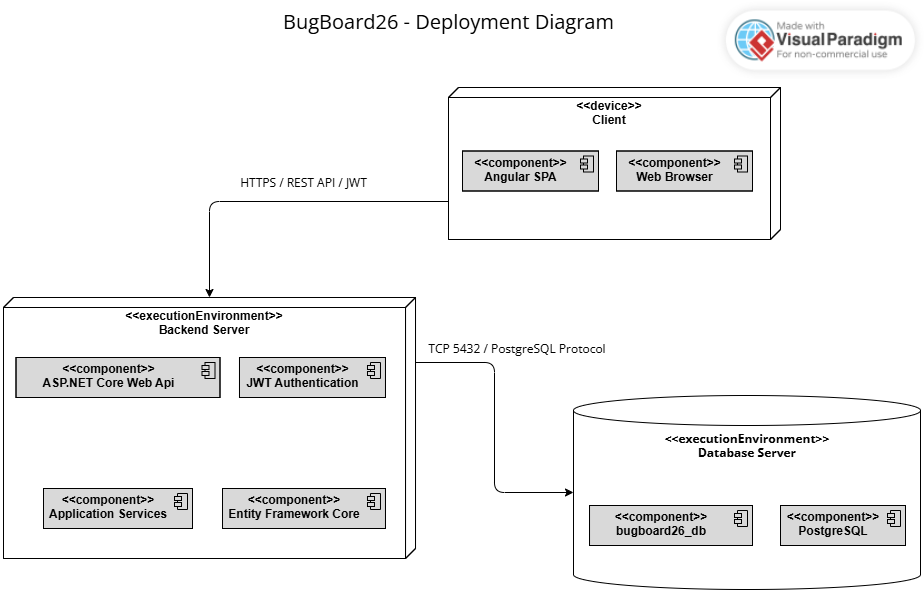
\includegraphics[width=0.85\textwidth]{diagrammi_architetturali/deployment_diagram.png}
    \caption{Deployment diagram di BugBoard26}
    \label{fig:deployment-diagram}
\end{figure}
}{
\begin{center}
    \fbox{\parbox{0.85\textwidth}{
        \centering
        Il file \texttt{diagrammi\_architetturali/deployment\_diagram.png} non è stato trovato.
    }}
\end{center}
}

La separazione in nodi distinti consente di eseguire le componenti in modo indipendente. In ambiente di sviluppo il database viene eseguito tramite Docker, mentre frontend e backend possono essere avviati separatamente. In una futura distribuzione, anche il backend e il frontend potrebbero essere eseguiti in container dedicati.

\clearpage
\section{Scelte tecnologiche}

\subsection{Frontend Angular}

Angular è stato scelto per realizzare una Single Page Application strutturata in componenti. Questa tecnologia permette di separare la presentazione dalla logica di accesso alle API e offre strumenti già integrati per routing, form, servizi e gestione delle chiamate HTTP.

Nel frontend sono previsti componenti dedicati alle principali schermate:

\begin{itemize}
    \item login;
    \item lista issue;
    \item creazione issue;
    \item dettaglio issue;
    \item archivio issue;
    \item notifiche;
    \item gestione utenti per amministratori.
\end{itemize}

\subsection{Backend ASP.NET Core Web API}

ASP.NET Core Web API è stato scelto per il backend perché supporta in modo nativo la creazione di API REST, la gestione della dependency injection, la autenticazione JWT e la integrazione con Entity Framework Core.

Il backend è organizzato secondo una struttura a livelli:

\begin{itemize}
    \item \textbf{Controller}: espongono gli endpoint REST;
    \item \textbf{Service}: contengono la logica applicativa;
    \item \textbf{Repository}: isolano lo accesso ai dati;
    \item \textbf{DbContext}: rappresenta il collegamento con il database.
\end{itemize}

Questa struttura consente di separare le responsabilità e rende più semplice testare la logica applicativa.

\subsection{Database PostgreSQL}

PostgreSQL è stato scelto come database relazionale per la persistenza delle informazioni principali del sistema. Le entità principali sono utenti, issue e notifiche.

La scelta di un database relazionale è coerente con la natura dei dati, che presentano relazioni chiare tra utenti, issue e notifiche.

\subsection{Autenticazione JWT}

La autenticazione è basata su token JWT. Dopo il login, il backend restituisce un token contenente le informazioni essenziali dello utente, tra cui identificativo e ruolo. Il frontend invia il token nelle richieste successive verso le API protette.

Questa soluzione permette di mantenere il backend stateless rispetto alle sessioni e di gestire in modo semplice autorizzazioni basate sui ruoli.

\section{Organizzazione del backend}

Il backend è stato progettato separando le responsabilità in più livelli.

\subsection{Controller}

I controller rappresentano il punto di ingresso delle richieste HTTP. Ogni controller espone un gruppo di API legate a una specifica area funzionale:

\begin{itemize}
    \item \texttt{AuthController}: login e generazione del token JWT;
    \item \texttt{UsersController}: creazione e consultazione degli utenti;
    \item \texttt{IssuesController}: creazione, ricerca, filtro, cambio stato, archiviazione, duplicati ed export;
    \item \texttt{NotificationsController}: consultazione e lettura delle notifiche.
\end{itemize}

\subsection{Servizi applicativi}

I servizi contengono la logica del sistema. In questo modo i controller rimangono semplici e si limitano a ricevere le richieste e restituire le risposte.

I principali servizi previsti sono:

\begin{itemize}
    \item \texttt{AuthService};
    \item \texttt{UserService};
    \item \texttt{IssueService};
    \item \texttt{NotificationService};
    \item \texttt{AssignmentSuggestionService};
    \item \texttt{CsvExportService}.
\end{itemize}

\subsection{Repository}

I repository isolano la logica di accesso ai dati. I servizi dipendono dalle interfacce dei repository e non direttamente dalla implementazione concreta. Questa scelta rende il sistema più testabile, poiché nei test è possibile sostituire i repository con implementazioni fittizie.

\subsection{DbContext}

\texttt{AppDbContext} rappresenta il punto di integrazione con Entity Framework Core. Al suo interno sono dichiarati i \texttt{DbSet} principali:

\begin{itemize}
    \item \texttt{Users};
    \item \texttt{Issues};
    \item \texttt{Notifications}.
\end{itemize}

\clearpage
\section{Class diagram di design}

Per migliorare la leggibilità, il class diagram è stato suddiviso in due viste complementari. La prima descrive il dominio e la persistenza, mentre la seconda mostra servizi, repository e dipendenze principali.

\subsection{Vista dominio e persistenza}

La vista dominio e persistenza mostra le entità principali del sistema e le relazioni tra esse.

\IfFileExists{diagrammi_dettaglio/class_diagram_parte1.png}{
\begin{figure}[H]
    \centering
    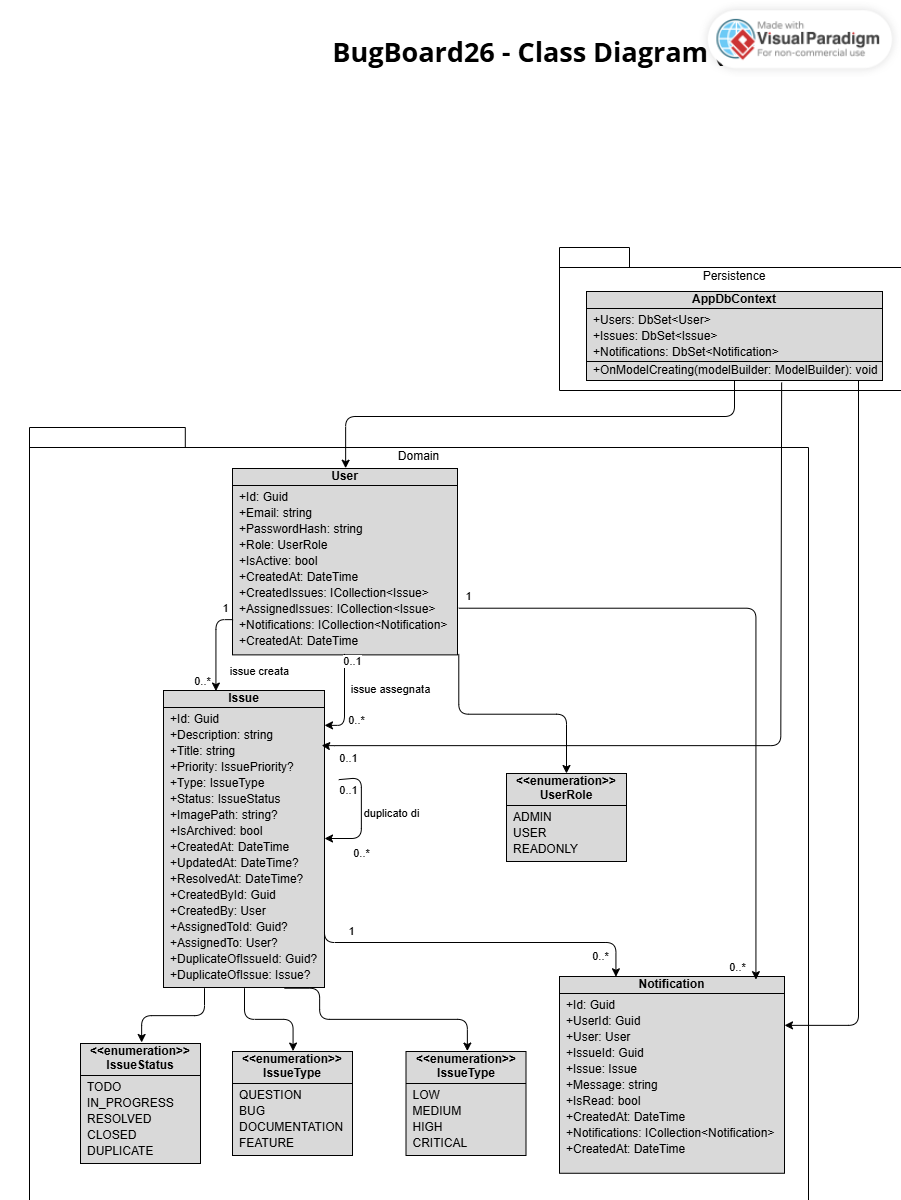
\includegraphics[
        width=0.95\textwidth,
        height=0.72\textheight,
        keepaspectratio
    ]{diagrammi_dettaglio/class_diagram_parte1.png}
    \caption{Class diagram: dominio e persistenza}
    \label{fig:class-domain-persistence}
\end{figure}
}{
\begin{center}
    \fbox{\parbox{0.85\textwidth}{
        \centering
        Il file \texttt{diagrammi_dettaglio/class_diagram_parte1.png} non è stato trovato.
    }}
\end{center}
}

Le entità principali sono \texttt{User}, \texttt{Issue} e \texttt{Notification}. Una issue è creata da uno utente e può essere assegnata a uno utente. Una issue può inoltre essere marcata come duplicata di un altra issue. Le notifiche sono associate sia allo utente destinatario sia alla issue di riferimento.

\subsection{Vista servizi e repository}

La vista servizi e repository mostra la organizzazione della logica applicativa del backend.

\IfFileExists{diagrammi_dettaglio/class_diagram_parte2.png}{
\begin{figure}[H]
    \centering
    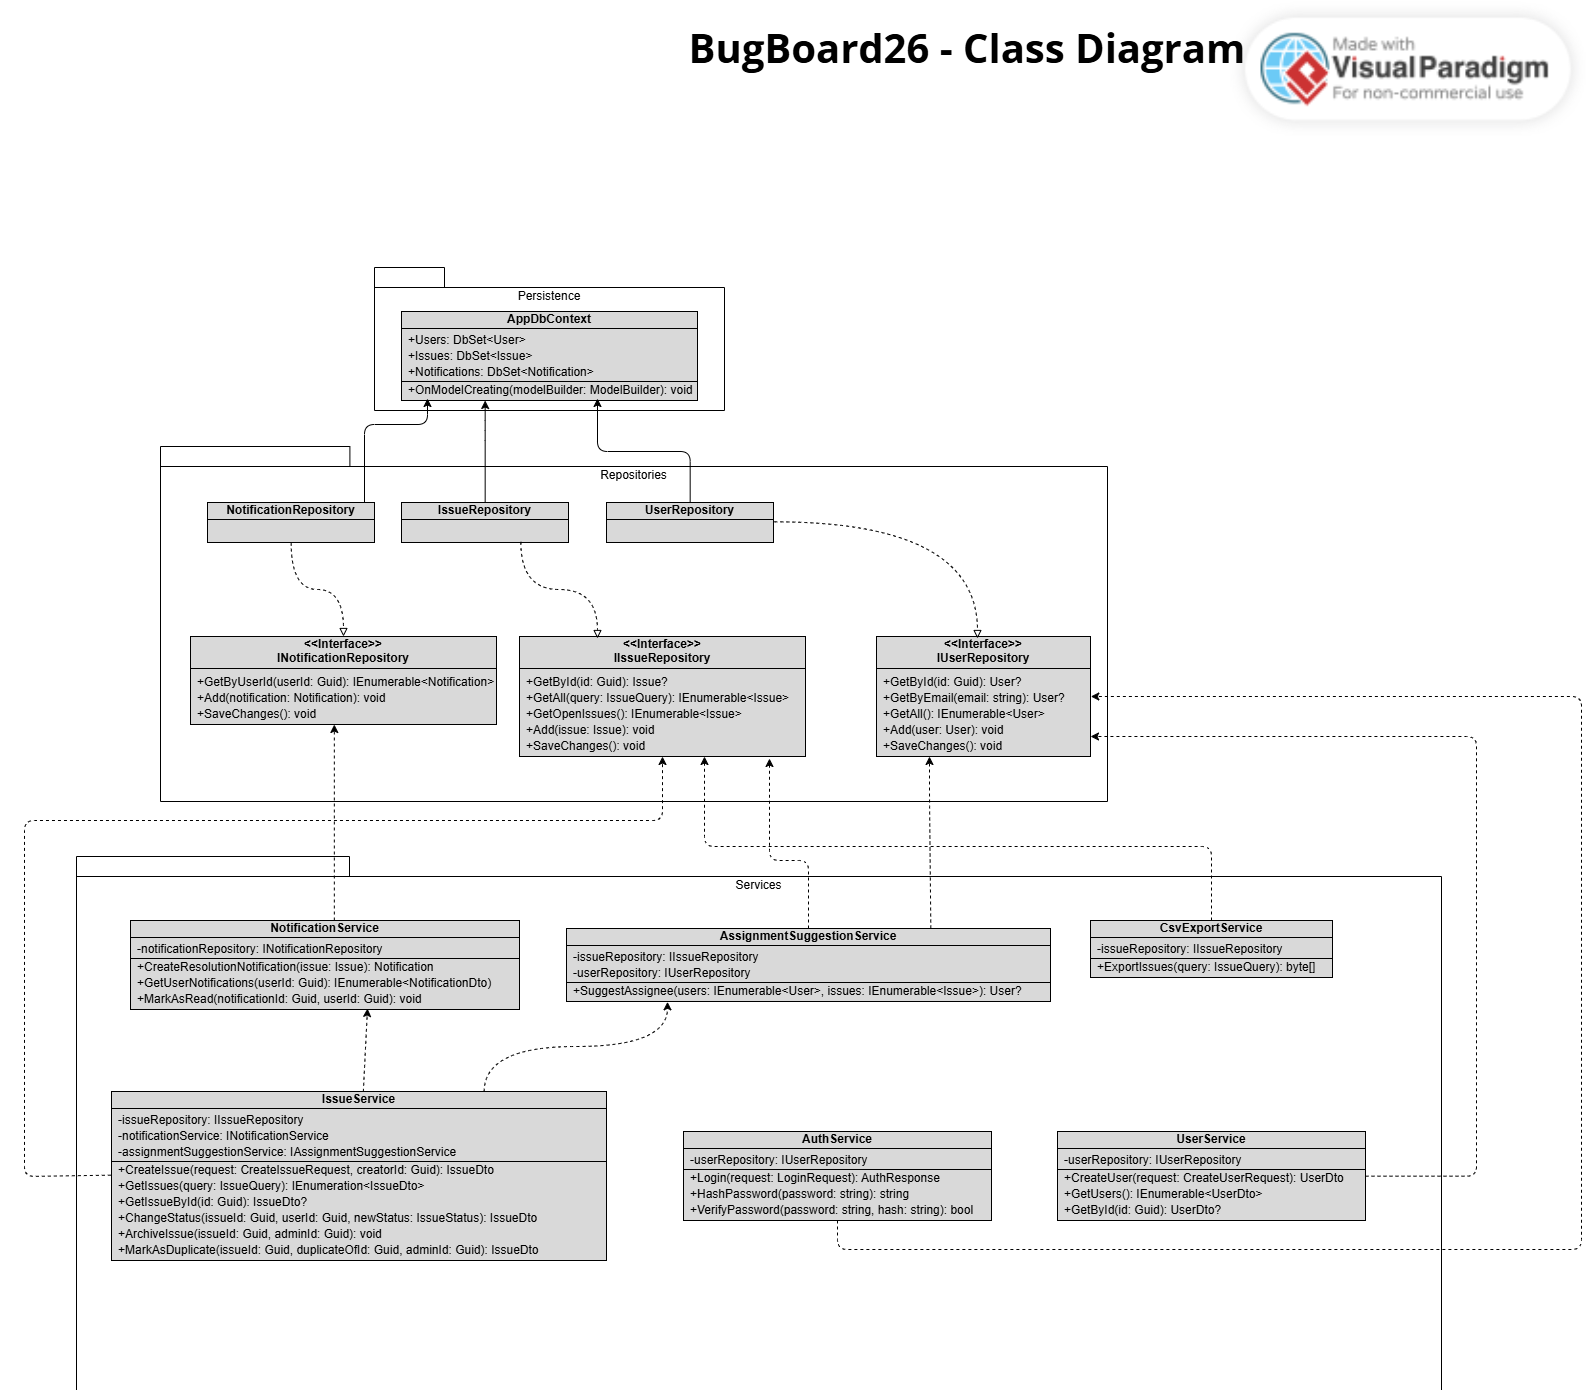
\includegraphics[width=0.95\textwidth]{diagrammi_dettaglio/class_diagram_parte2.png}
    \caption{Class diagram: servizi e repository}
    \label{fig:class-services-repositories}
\end{figure}
}{
\begin{center}
    \fbox{\parbox{0.85\textwidth}{
        \centering
        Il file \texttt{diagrammi_dettaglio/class_diagram_parte2.png} non è stato trovato.
    }}
\end{center}
}

I servizi applicativi utilizzano le interfacce dei repository per accedere ai dati. Le classi concrete dei repository implementano tali interfacce e usano \texttt{AppDbContext}. Questa struttura riduce lo accoppiamento tra logica applicativa e persistenza.

\clearpage
\section{Schema della persistenza dati}

La persistenza dei dati è basata su tre tabelle principali:

\begin{itemize}
    \item \texttt{Users};
    \item \texttt{Issues};
    \item \texttt{Notifications}.
\end{itemize}

\IfFileExists{diagrammi_dettaglio/database_schema.png}{
\begin{figure}[H]
    \centering
    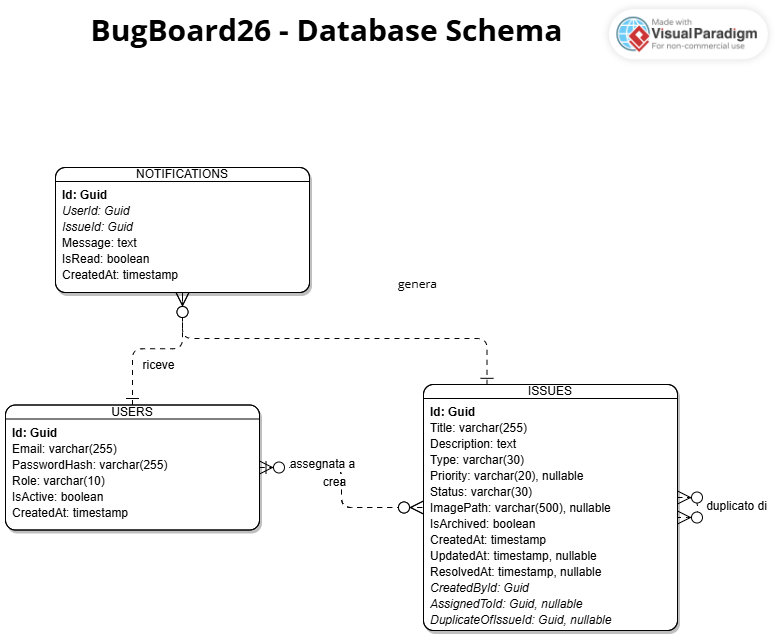
\includegraphics[width=0.95\textwidth]{diagrammi_dettaglio/database_schema.png}
    \caption{Schema della persistenza dati}
    \label{fig:database-schema}
\end{figure}
}{
\begin{center}
    \fbox{\parbox{0.85\textwidth}{
        \centering
        Il file \texttt{diagrammi\_dettaglio/database\_schema.png} non è stato trovato. Lo schema può essere aggiunto dopo la definizione finale delle migration.
    }}
\end{center}
}

\begin{longtable}{p{0.22\textwidth} p{0.68\textwidth}}
\toprule
\textbf{Tabella} & \textbf{Descrizione} \\
\midrule
\endhead
\texttt{Users} & Contiene gli utenti del sistema, le credenziali cifrate tramite hash, il ruolo e lo stato di attivazione. \\
\texttt{Issues} & Contiene le issue create dagli utenti, il loro stato, la priorità, il tipo, lo assegnatario, le informazioni di archiviazione e lo eventuale collegamento a una issue duplicata. \\
\texttt{Notifications} & Contiene le notifiche generate dal sistema, in particolare quelle relative alla risoluzione di una issue. \\
\bottomrule
\end{longtable}

\section{Principali scelte di design}

\subsection{Separazione frontend e backend}

Il frontend non accede direttamente al database e non contiene logica di business critica. Tutte le regole principali, come controllo dei ruoli, cambio stato, archiviazione e gestione dei duplicati, sono implementate nel backend.

\subsection{Uso di servizi applicativi}

La logica applicativa è concentrata nei servizi. Questa scelta permette di mantenere i controller più semplici e di testare più facilmente le operazioni principali.

\subsection{Uso di repository}

I repository sono stati introdotti per separare la logica applicativa dallo accesso ai dati. I servizi dipendono da interfacce, non da implementazioni concrete. Questo favorisce testabilità e sostituibilità delle implementazioni.

\subsection{Gestione dei ruoli}

Il sistema prevede tre ruoli principali:

\begin{itemize}
    \item \texttt{ADMIN}: può gestire utenti, archiviare issue, esportare dati e contrassegnare duplicati;
    \item \texttt{USER}: può creare issue, consultarle e cambiare lo stato delle issue assegnate;
    \item \texttt{READONLY}: può solo consultare le issue, senza modificarle.
\end{itemize}

Il controllo dei ruoli viene effettuato lato backend, in modo da impedire operazioni non autorizzate anche in caso di manipolazione della interfaccia frontend.

\subsection{Suggerimento automatico dello assegnatario}

Il suggerimento automatico dello assegnatario è realizzato considerando il carico di lavoro corrente degli utenti. Il criterio di base è selezionare lo utente normale con il minor numero di issue aperte assegnate.

Le issue risolte, duplicate o archiviate non vengono considerate come carico attivo. In caso di parità è possibile scegliere un criterio stabile, per esempio ordinamento per email.

\subsection{Gestione delle notifiche}

Quando una issue viene portata allo stato \texttt{RESOLVED}, il sistema genera una notifica per lo utente che ha creato la issue. La notifica viene salvata nel database e può essere visualizzata dalla interfaccia utente.

\clearpage
\subsection{Gestione dei duplicati}

Solo gli amministratori possono contrassegnare una issue come duplicata. Quando questo avviene, la issue viene collegata a una issue principale e il suo stato viene impostato a \texttt{DUPLICATE}. In questo modo rimane tracciabile ma non viene più considerata come issue aperta da risolvere.

\subsection{Archiviazione}

Solo gli amministratori possono archiviare una issue. Una issue archiviata non viene mostrata nella lista principale, ma resta accessibile da una sezione dedicata. Questa scelta permette di non eliminare dati utili e di conservare la tracciabilità delle segnalazioni.

\section{Diagrammi comportamentali}

I diagrammi comportamentali descrivono il flusso delle interazioni tra frontend, controller, servizi, repository e database per alcune funzionalità centrali del sistema. Sono stati scelti i casi relativi alla creazione di una issue, al cambio stato con generazione della notifica e alla gestione dei duplicati, perché rappresentano parti significative della logica applicativa.

\subsection{Creazione di una issue}

\begin{figure}[H]
    \centering
    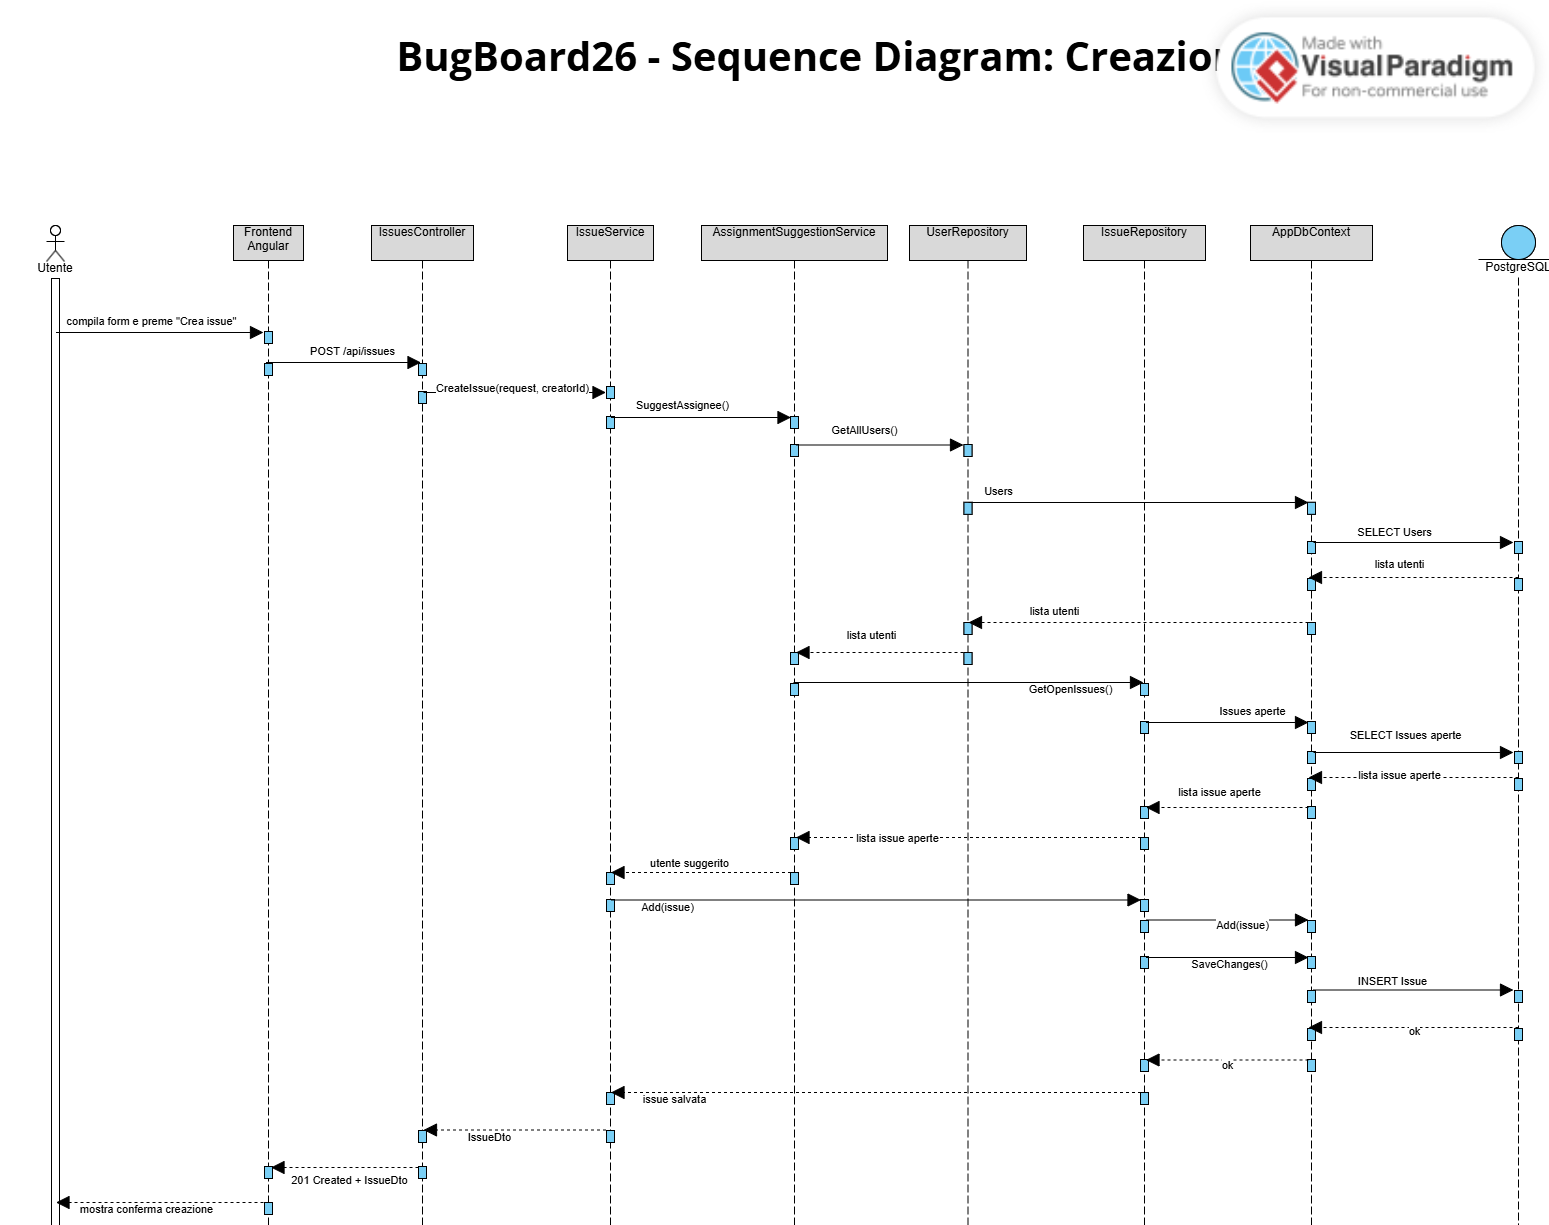
\includegraphics[
        width=0.95\textwidth,
        height=0.70\textheight,
        keepaspectratio
    ]{diagrammi_comportamentali/sequence_creazione_issue.png}
    \caption{Sequence diagram: creazione di una issue}
    \label{fig:sequence-creazione-issue}
\end{figure}

\subsection{Cambio stato con notifica}

\begin{figure}[H]
    \centering
    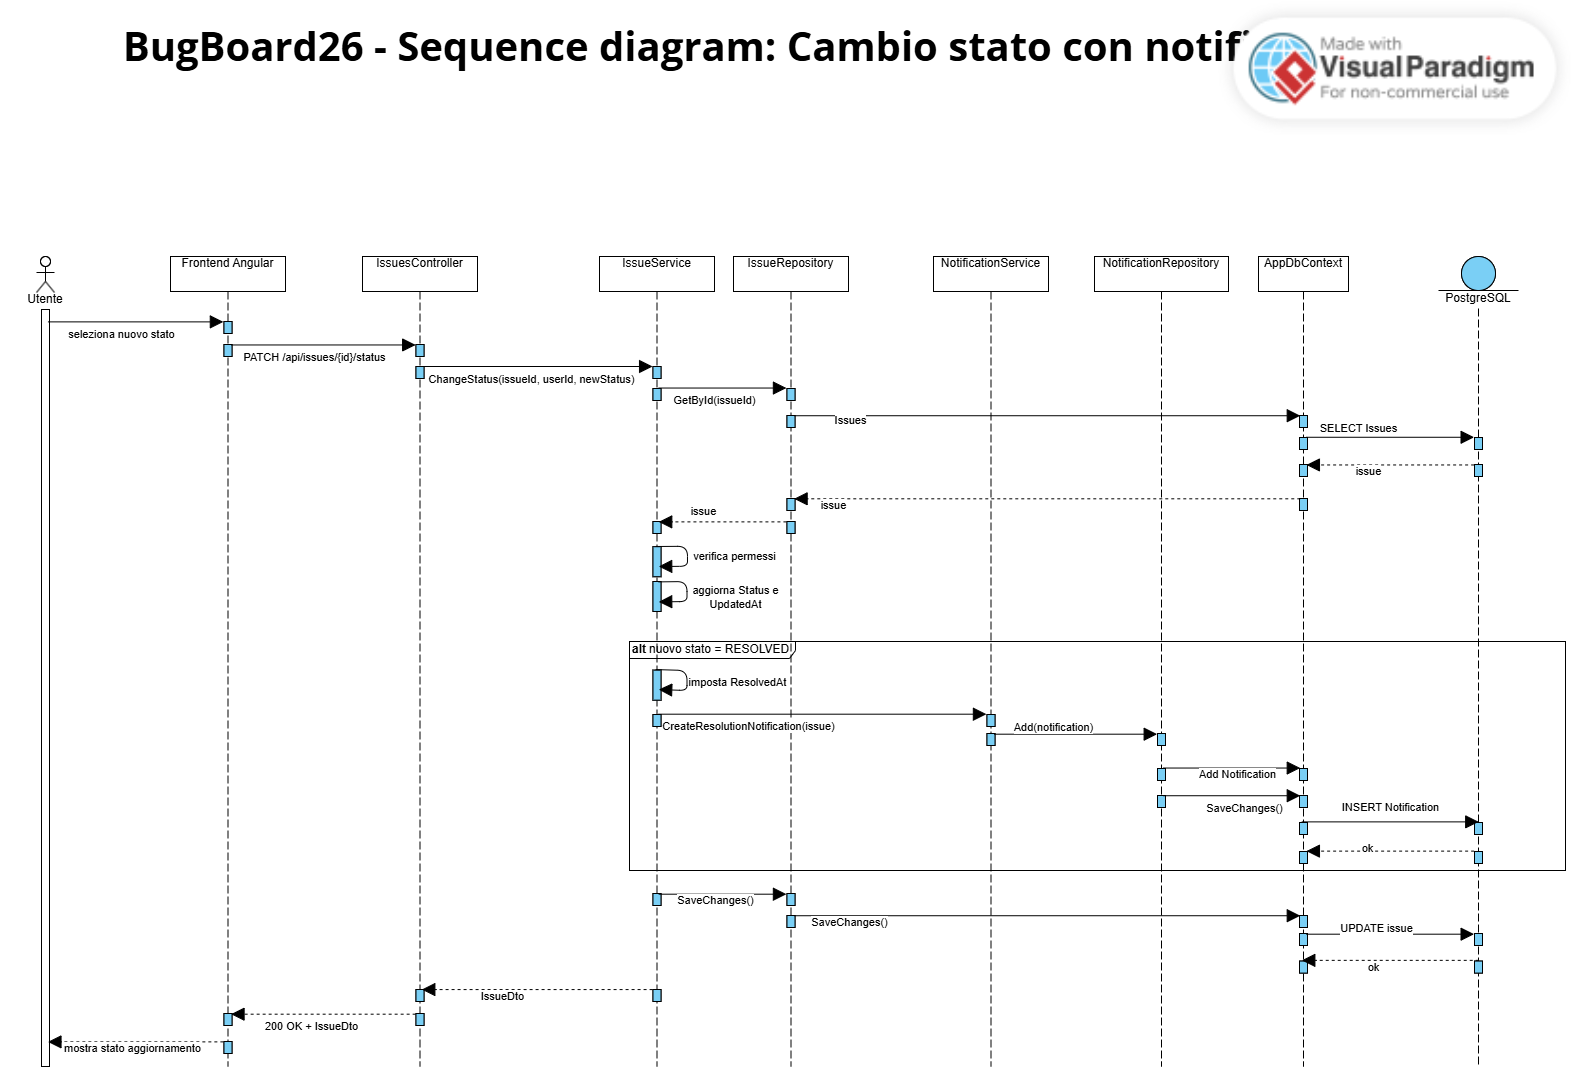
\includegraphics[
        width=0.85\textwidth,
        height=0.60\textheight,
        keepaspectratio
    ]{diagrammi_comportamentali/sequence_cambio_stato.png}
    \caption{Sequence diagram: cambio stato con notifica}
    \label{fig:sequence-cambio-stato-notifica}
\end{figure}

\subsection{Contrassegno di una issue duplicata}

\begin{figure}[H]
    \centering
    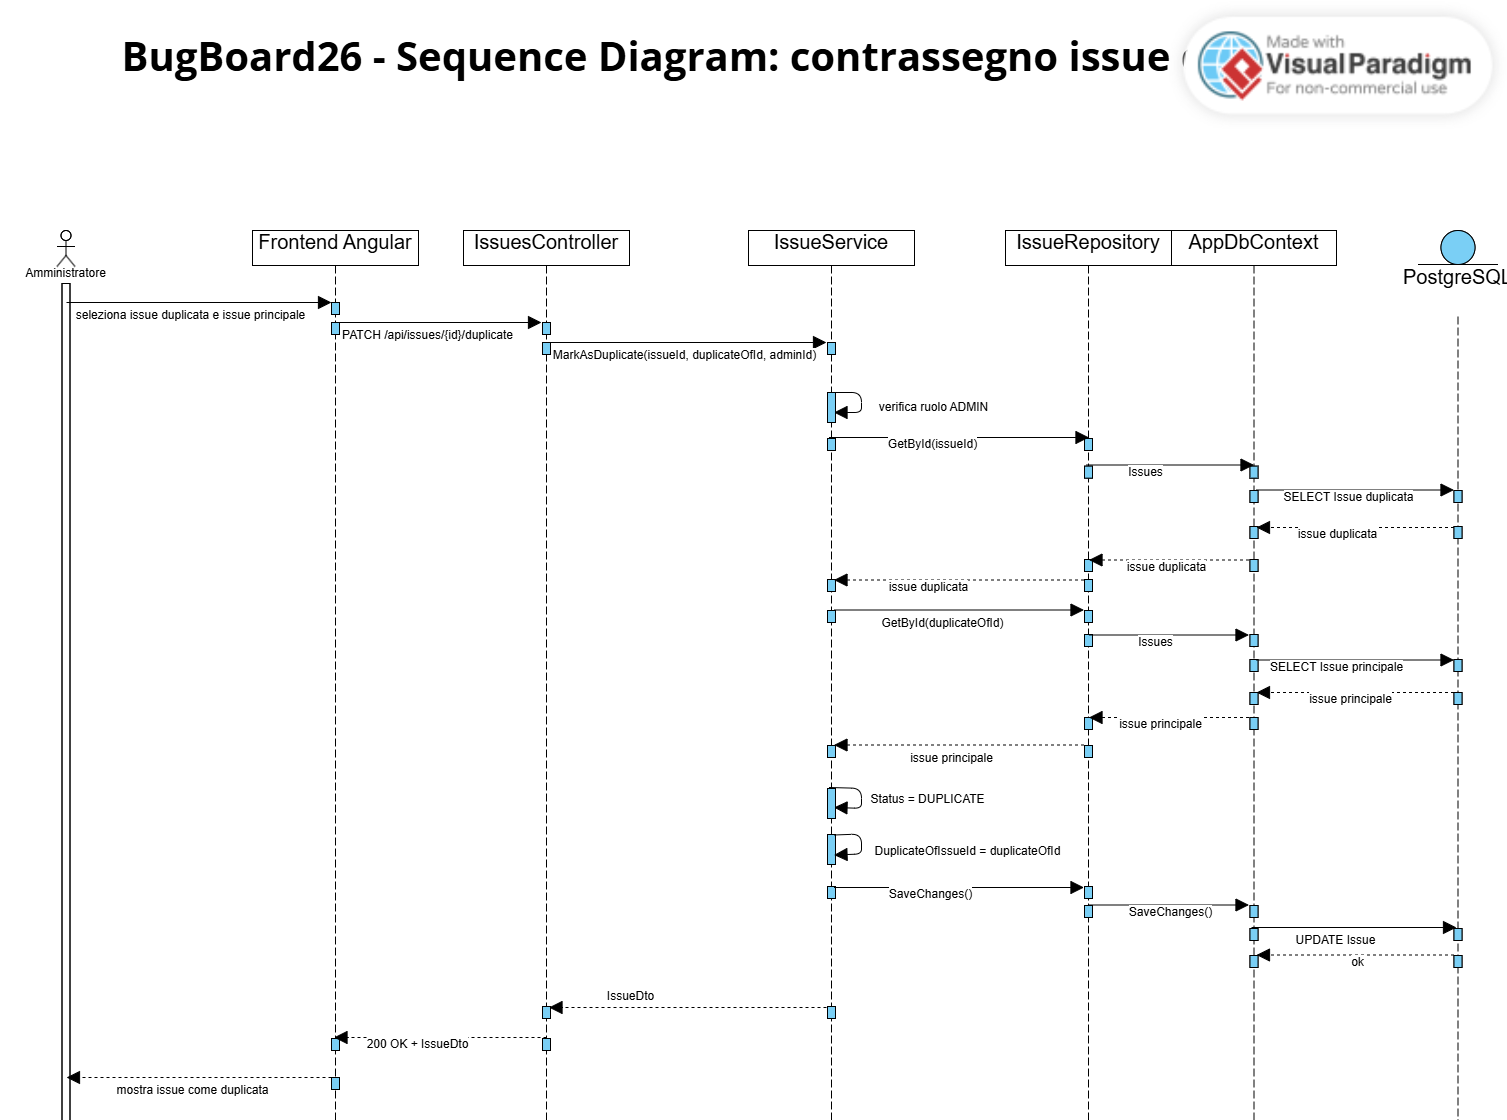
\includegraphics[
        width=0.85\textwidth,
        height=0.60\textheight,
        keepaspectratio
    ]{diagrammi_comportamentali/sequence_issue_duplicata.png}
    \caption{Sequence diagram: contrassegno di una issue duplicata}
    \label{fig:sequence-duplica-issue}
\end{figure}


\clearpage
\section{API principali previste}

\begin{table}[H]
\centering
\renewcommand{\arraystretch}{1.45}
\setlength{\extrarowheight}{3pt}

\begin{tabularx}{\textwidth}{
    L{0.13\textwidth}
    L{0.40\textwidth}
    X
}
\toprule
\textbf{Metodo} & \textbf{Endpoint} & \textbf{Descrizione} \\
\midrule
POST & \url{/api/auth/login} &
Effettua il login e restituisce il token JWT. \\
POST & \url{/api/users} &
Crea un nuovo utente. Operazione riservata agli amministratori. \\
GET & \url{/api/users} &
Restituisce la lista degli utenti. \\
POST & \url{/api/issues} &
Crea una nuova issue. \\
GET & \url{/api/issues} &
Restituisce le issue con ricerca, filtri e ordinamento. \\
GET & \url{/api/issues/\{id\}} &
Restituisce il dettaglio di una issue. \\
PATCH & \url{/api/issues/\{id\}/status} &
Modifica lo stato di una issue assegnata. \\
PATCH & \url{/api/issues/\{id\}/archive} &
Archivia una issue. Operazione riservata agli amministratori. \\
GET & \url{/api/issues/archived} &
Restituisce le issue archiviate. \\
PATCH & \url{/api/issues/\{id\}/duplicate} &
Contrassegna una issue come duplicata. \\
GET & \url{/api/issues/export} &
Esporta le issue in formato CSV. \\
GET & \url{/api/notifications} &
Restituisce le notifiche dell'utente autenticato. \\
PATCH & \url{/api/notifications/{id}/read} &
Segna una notifica come letta. \\

\bottomrule
\end{tabularx}
\caption{Endpoint principali esposti dal backend}
\label{tab:endpoint-backend}
\end{table}

\clearpage
\section{Testabilità}

La progettazione è stata impostata per rendere testabili le parti principali della logica applicativa. In particolare, i servizi non dipendono direttamente dal database, ma dalle interfacce dei repository. Questo consente di testare i servizi usando dati controllati.

Le funzionalità più adatte ai test automatici sono:

\begin{itemize}
    \item suggerimento dello assegnatario;
    \item verifica dei permessi per il cambio stato;
    \item ricerca e filtro delle issue;
    \item generazione della notifica alla risoluzione;
    \item gestione del duplicato.
\end{itemize}

\section{Conclusioni}

La progettazione proposta divide BugBoard26 in componenti indipendenti e con responsabilità chiare. Il frontend Angular si occupa della presentazione, il backend ASP.NET Core contiene la logica applicativa e PostgreSQL gestisce la persistenza dei dati.

La struttura a livelli adottata rende il sistema più ordinato, testabile ed estendibile. Le scelte di design sono coerenti con le funzionalità assegnate e con il vincolo di realizzare un sistema distribuito con frontend e backend separati.

\end{document}
